\documentclass[11pt, a4paper]{article}
%-------------
% SETTINGS
%-------------
	\usepackage{enumitem,amsmath,amsthm,amssymb,stmaryrd,amsfonts,graphicx,subfig,footnote,float,caption}
	\captionsetup{justification=centering, font=footnotesize, skip=1pt}
	\usepackage[dvipsnames]{xcolor}
    \usepackage{array,multirow,colortbl,diagbox}
	\usepackage{microtype,float}
	\newfloat{listing}{tbhp}{lst}%[section]
	\floatname{listing}{Stdout}
	\usepackage[left=2cm,right=2cm,top=2.5cm,bottom=2cm]{geometry}
	\usepackage{hyperref}
	\graphicspath{{../figures/}}
	\setlength{\parindent}{0cm}
%	\renewcommand*{\thefootnote}{(*)}
	\renewcommand{\baselinestretch}{1.2}
	\setlength{\headheight}{13.6pt}
    \newcommand{\cg}{\cellcolor{gray!70}}
%-----------------------
% TIKZ
% -----------------------
    \usepackage{tikz}
    \usetikzlibrary{arrows,positioning}
    \tikzstyle{state}=[draw, fill=white, align=center]
    \tikzstyle{sum}=[draw, circle, fill=white, align=center, inner sep=1,outer sep=0]

%------------------------
% MATH
% -----------------------
	\newcommand{\p}{\mathbb{P}}
	\newcommand{\Q}{\mathbf{Q}}
	\newcommand{\W}{\mathbf{W}}
    \renewcommand{\theequation}{Eq\arabic{equation}}


%-------------
% TITLE
%-------------
	\author{Maha Elbayad}
	\title{Foundations of Machine Learning II \\Project: Bandits and Wumpus}
	\date{}
%------------------------
% CONTENT
% -----------------------


\begin{document}
\maketitle
\subsection*{Question 1}
It's interesting to give negative reward to the default event so that we encourage the agent to look for rewarding states and actions.
\subsection*{Question 2}
We run the random agent and track the duration and the cumulative reward at the end of each episode (figure~\ref{rdm}). We note that the cumulative reward is in fact random with a high standard deviation $\approx 55$ and two distinctive modes: a very large reward or a very large penalty.


\subsection*{Question 3}
We implemented an agent that uses its flash units wisely i.e only when it receives a smell signal and then moves into the same direction after flashing.

The prudent agent performs slightly better than the random agent:
\begin{listing}
\begin{verbatim}
Average reward/step for "random": 2.20
Average cumulative reward/episode for "random": 25.79
Average reward/step for "Prudent": 3.65
Average cumulative reward/episode for "Prudent": 30.52
\end{verbatim}
\caption{Statistics during 100 episodes}
\end{listing}

\begin{figure}[H]
\centering
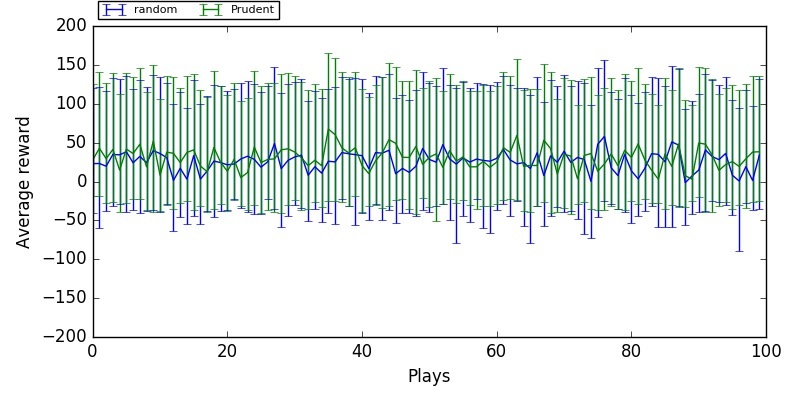
\includegraphics[width=14cm]{randPrud}
\caption{Random and Prudent agents performance - YAxis: the episode average reward\label{rdm}}
\end{figure}

\subsection*{Question 4}
The major drawback of the greedy strategy is that the agent would rather exploit its discoveries than keep looking for an optimal path. e.g. in the default grid the agent keep repeating the path (0,0)-up-(3,0)-left-(3,3) which is a local optimum. 


\subsection*{Question 5: Implementation}
We experiment with 3 different state spaces \{\texttt{BSF, ABSF, XYBSF}\} and variant parameters ($\epsilon$ for the greedy agent and the temperature $\tau$ for the softmax agent) - the curves below take into account the results of 20 runs of 100 episode/play each.
\paragraph{The sate encoding:}
When enriching the state space especially with the location parameters the greedy agent outperforms the rest.

\paragraph{Greedy algorithm:}
The greedy agent ($\epsilon \approx 0$) improved slightly faster than the others at first, but then leveled off at a lower level (sort of local optimum). Moreover, the greedy runs are sensitive to those initial steps where for a given state $s$, $\max Q(a,s)$ is achieved at multiple actions, between figure 2 and figure 3 the greedy performance is quite instable.

\paragraph{Softmax algorithm:}
Low temperature values yields agents similar to the greedy while large temperatures render the states equiprobable.
\subsubsection*{BSF}
\begin{listing}
\begin{verbatim}
Average reward/step for "BSF eps-Greedy (0.01)": -0.57
Average cumulative reward/episode for "BSF eps-Greedy (0.01)": -99.42
Average reward/step for "BSF eps-Greedy (0.1)": 1.48
Average cumulative reward/episode for "BSF eps-Greedy (0.1)": 36.55
Average reward/step for "BSF eps-Greedy (0.3)": 3.03
Average cumulative reward/episode for "BSF eps-Greedy (0.3)": 38.60
\end{verbatim}
\caption{Statistics for 100 episodes $\epsilon$-Greedy BSF}
\end{listing}


\begin{figure}[H]
\centering
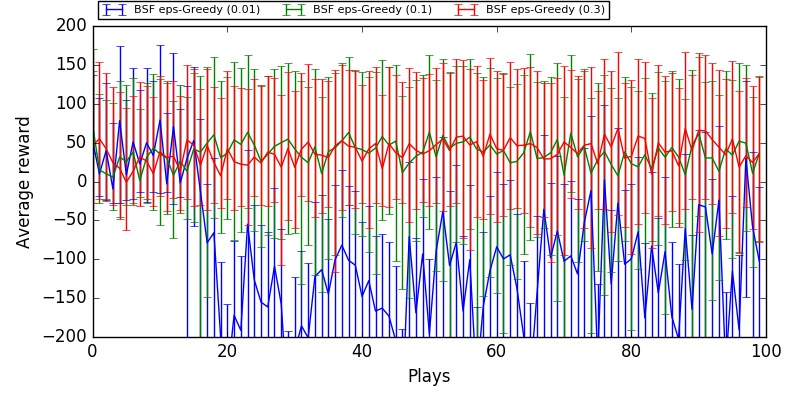
\includegraphics[width=14cm]{BSF_eps_Learning}
\caption{BSF - $\epsilon$-Greedy (run2)}
\end{figure}

\subsubsection*{ABSF}
\begin{listing}
\begin{verbatim}
Average reward/step for "ABSF eps-Greedy (0.01)": 0.76
Average cumulative reward/episode for "ABSF eps-Greedy (0.01)": 28.94
Average reward/step for "ABSF eps-Greedy (0.1)": 6.36
Average cumulative reward/episode for "ABSF eps-Greedy (0.1)": 56.34
Average reward/step for "ABSF eps-Greedy (0.3)": 6.12
Average cumulative reward/episode for "ABSF eps-Greedy (0.3)": 49.51
\end{verbatim}
\caption{Statistics for 100 episodes $\epsilon$-Greedy ABSF}
\end{listing}

\begin{figure}[H]
\centering
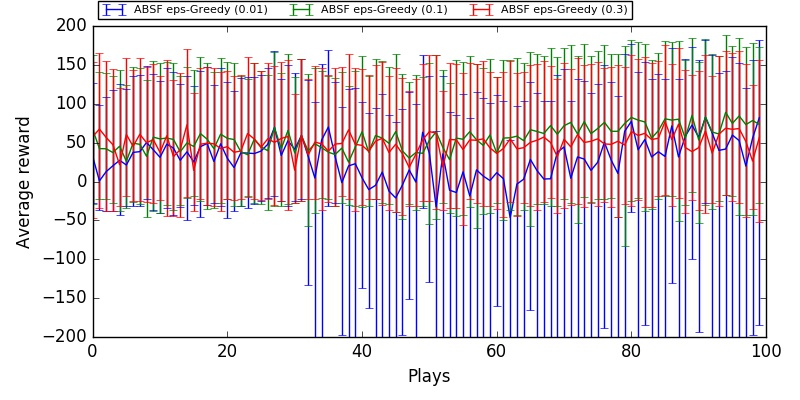
\includegraphics[width=14cm]{ABSF_eps_Learning}
\caption{ABSF - $\epsilon$-Greedy}
\end{figure}

\subsubsection*{XYBSF}
\begin{listing}
\begin{verbatim}
Average reward/step for "XYBSF eps-Greedy (0.01)": 15.61
Average cumulative reward/episode for "XYBSF eps-Greedy (0.01)": 85.22
Average reward/step for "XYBSF eps-Greedy (0.1)": 12.15
Average cumulative reward/episode for "XYBSF eps-Greedy (0.1)": 75.88
Average reward/step for "XYBSF eps-Greedy (0.3)": 8.62
Average cumulative reward/episode for "XYBSF eps-Greedy (0.3)": 61.08
\end{verbatim}
\caption{Statistics for 100 episodes $\epsilon$-Greedy XYBSF}
\end{listing}

\begin{figure}[H]
\centering
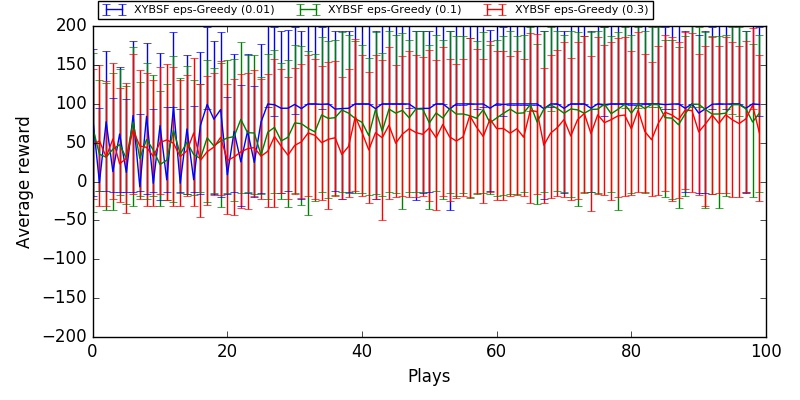
\includegraphics[width=14cm]{XYBSF_eps_Learning}
\caption{XYBSF $\epsilon$-Greedy}
\end{figure}
%%%%%%%%%%%%%%%%%%%%%%%%%%%
%%
%%      Softmax
%%
%%%%%%%%%%%%%%%%%%%%%%%%%%%%%
\subsubsection*{BSF}
\begin{listing}
\begin{verbatim}
Average reward/step for "BSF Softmax (1)": 1.85
Average cumulative reward/episode for "BSF Softmax (1)": 40.80
Average reward/step for "BSF Softmax (3)": 3.30
Average cumulative reward/episode for "BSF Softmax (3)": 42.26
Average reward/step for "BSF Softmax (10)": 3.16
Average cumulative reward/episode for "BSF Softmax (10)": 36.73
\end{verbatim}
\caption{Statistics for 100 episodes Softmax - BSF}
\end{listing}


\begin{figure}[H]
\centering
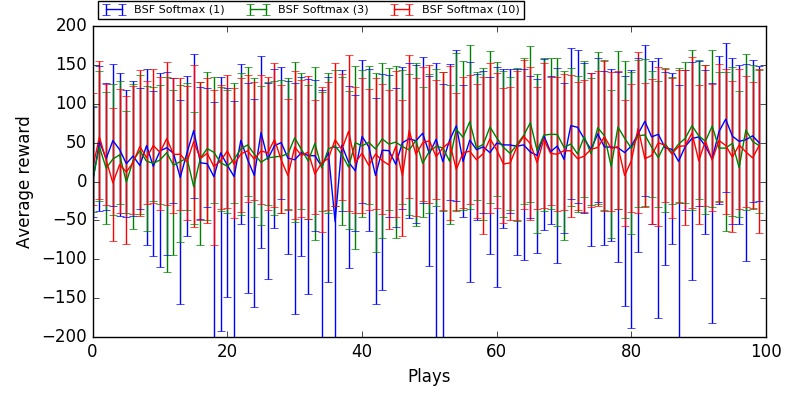
\includegraphics[width=14cm]{BSF_sfmax_Learning}
\caption{BSF - softmax}
\end{figure}


\subsubsection*{ABSF}
\begin{listing}
\begin{verbatim}
Average reward/step for "ABSF Softmax (1)": 7.06
Average cumulative reward/episode for "ABSF Softmax (1)": 56.72
Average reward/step for "ABSF Softmax (3)": 6.62
Average cumulative reward/episode for "ABSF Softmax (3)": 56.10
Average reward/step for "ABSF Softmax (10)": 4.53
Average cumulative reward/episode for "ABSF Softmax (10)": 44.79
\end{verbatim}
\caption{Statistics for 100 episodes Softmax - ABSF}
\end{listing}

\begin{figure}[H]
\centering
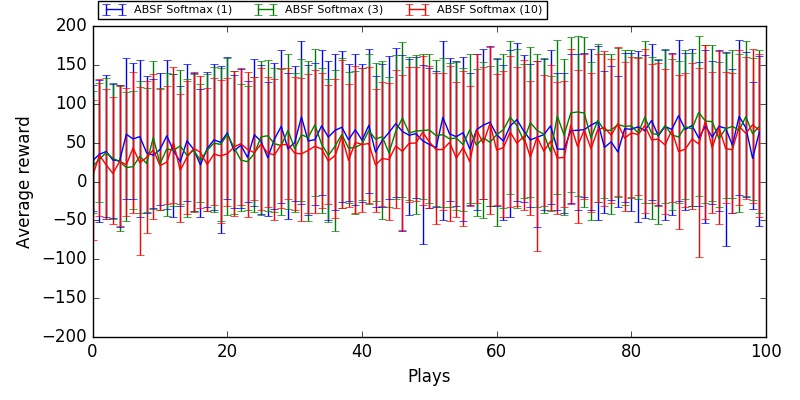
\includegraphics[width=14cm]{ABSF_sfmax_Learning}
\caption{ABSF - softmax}
\end{figure}

\subsubsection*{XYBSF}
\begin{listing}
\begin{verbatim}
Average reward/step for "XYBSF Softmax (1)": 8.66
Average cumulative reward/episode for "XYBSF Softmax (1)": 70.39
Average reward/step for "XYBSF Softmax (3)": 7.93
Average cumulative reward/episode for "XYBSF Softmax (3)": 68.15
Average reward/step for "XYBSF Softmax (10)": 8.02
Average cumulative reward/episode for "XYBSF Softmax (10)": 64.43
\end{verbatim}
\caption{Statistics for 100 episodes Softmax - XYBSF}
\end{listing}

\begin{figure}[H]
\centering
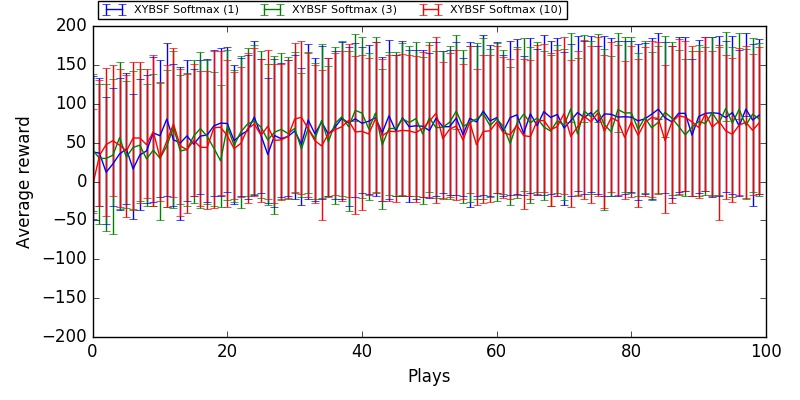
\includegraphics[width=14cm]{XYBSF_sfmax_Learning}
\caption{XYBSF - softmax}
\end{figure}


\subsection*{Qestion 7 : UCB}
The next agent aims at maximizing the Upper Confidence Bound Confidence (UCB), we compare the two encodings ABSF and XYBSF with the random agent:
\begin{listing}
\begin{verbatim}
Average reward/step for "XYBSF UCB": 4.33
Average cumulative reward/episode for "XYBSF UCB": 46.38
Average reward/step for "ABSF UCB": 4.02
Average cumulative reward/episode for "ABSF UCB": 41.56
Average reward/step for "random": 2.08
Average cumulative reward/episode for "random": 24.12
\end{verbatim}
\caption{Statistics for 100 episodes Softmax - XYBSF}
\end{listing}

\begin{figure}[H]
\centering
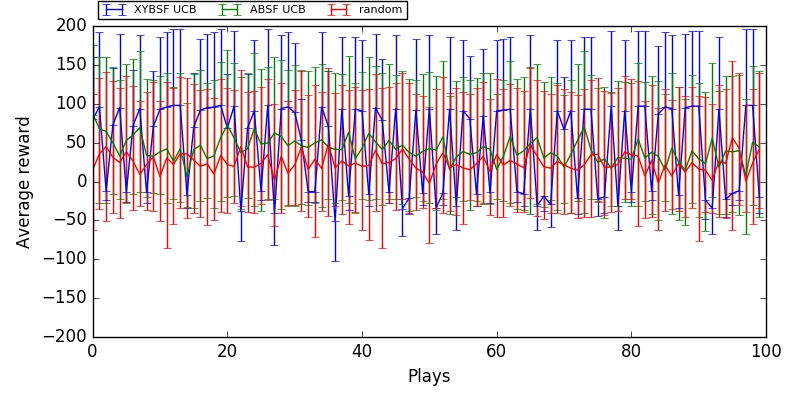
\includegraphics[width=14cm]{UCB}
\caption{}
\end{figure}
\end{document}